\RequirePackage[orthodox]{nag}
\documentclass[11pt]{article}

%% Define the include path
\makeatletter
\providecommand*{\input@path}{}
\g@addto@macro\input@path{{include/}{../../include/}}
\makeatother

\usepackage{../../include/akazachk}

\title{Operations Research}
\author{Andres Espinosa}
\begin{document}
\pgfplotsset{compat=1.18}
\maketitle

\tableofcontents
\section{Wednesday April 22nd}
\subsection{Exercises}
\subsubsection{Graph Question 4}

Show that a connected graph has at least $n-1$ edges.

In the best case scenario, if we build a graph starting from one node, in order to connect it we would like to connect it and reduce the number of connected components by one each time.
Therefore, $C(G_{n}) = C(G_{n-1}) -1  = n - 1$
A tree, which has no cycles and is connected, must have exactly $n-1$ edges.

\subsubsection{Algorithm 1}
Prove: it is always possible to extract, from a (directed) path going from $i$ to $j$, a simple path going from $i$ to $j$.

A simple path is defined as a path where no node is visited more than once.
Effectively, from any path, that can contain cycles, it is possible to create an acyclic path.
For any cycle, we can have the same path but exit the cycle at the node previous to the cycling node.
For a cycle and a path entering that cycle, we can define the nodes $N_i, N_o, N_c$ as the input, output, and cycling node.
We can always take the node that feeds into the cycline node $N_c-1$, and use that as the node to feed into the output.

\subsubsection{Algorithm 2}
Determining the adjacency matrix, alpha, and beta for the graph

\begin{align}
  \textbf{A} = 
  \begin{bmatrix}
     1 & 1 & 1 & 1 & 0 \\
     1 & 0 & 1 & 0 & 0 \\
     0 & 0 & 0 & 0 & 0 \\
     0 & 0 & 0 & 0 & 1 \\
     0 & 0 & 1 & 1 & 0
  \end{bmatrix}
\end{align}

\begin{equation}
    \beta = [1, 2, 3, 4, 1, 3, 5, 3, 4]
\end{equation}
\begin{equation}
    \alpha = [1, 5, 7, 7, 8, 10]
\end{equation}

To extract the list of successors of a node $n$, we get the list $[\beta[\alpha[n]], \beta[\alpha[n+1] - 1]]$

\subsubsection{Bipartite}
For a bipartite and bicoloured graph, any green node can be reached from a starting red node in a path of odd length.
This is because for any node, it must be able to have been colored in a path with alternating colors.

\section{Thursday April 23rd}
\subsection{Scrap}
\subsubsection{Kruskal Algorithm Complexity}

\section{Friday April 24th}
\subsection{Puzzle Exercises}
\subsubsection{Lewis Carrol Puzzle}
\begin{enumerate}
    \item Yellow, Norwegian, Diplomat, Water, Fox
    \item  Blue, Italian, Doctor, Tea, Horse
    \item  Red, English, Sculptor, Milk, Snails
    \item  White, Spaniard, Violinist, Fruit Juice, Dog
    \item  Green, Japanese, Painter, Coffee, Zebra
\end{enumerate}

\subsubsection{Forty Ten Ten}
Forty + Ten + Ten = Sixty
\subsubsection{Send More Money}
Send + More = Money
\begin{gather}
    Send \\
    + More \\
    = Money
\end{gather}

\begin{gather}
    D + E = Y + 10 x_1 \\ 
    x_1 + N + R = E + 10 x_2 \\
    x_2 + E + O = N + 10 x_3 \\
    x_3 + S + M = O + 10 x_4 \\ 
    x_4 = M
\end{gather}
\begin{equation}
    M = 1
\end{equation}

\begin{equation}
    x_3 + S = O + 9
\end{equation}
Here, we split off between the possibility of $S=8,9$

\textbf{First Scenario:} $S=8$
\begin{gather}
    x_3 = O + 1 \\
    O = 0, x_3 = 1 \\
    x_2 + E = N + 10
\end{gather}
This is impossible because in this scenario, $0,1$ are both taken and therefore we can not get to 12

\textbf{Second Scenario:} $S=9$
\begin{gather}
    x_3 = O \\ 
    x_3 = 0, O = 0 \\
    x_2 + E = N \\
    N = E + 1
\end{gather}

$x_2=1$ because if it is zero then $E=N$, which we cannot have
\begin{gather}
    x_1 + E + 1 + R = E + 10 \\
    x_1 + R = 9
\end{gather}
Since $x_1$ is equal to 0 or 1, $R$ is either 8 or 9, which it isn't 9 since $S$ has already taken it.
$R=8, x_1 = 1$.


Here we will need to split off possible values of $E$.

\begin{gather}
    x_4 = 1, x_3 = 0, x_2 = 1, x_1 = 1 \\
    M = 1, O = 0, R = 8
\end{gather}

\textbf{First Scenario:} $E=2, N=3$
\begin{gather}
    E = 2, N = 3 \\
    D + 2 = Y + 10
    D  = Y + 8
\end{gather}
That can't be right, since 0 and 1 are taken so Y would have to be greater than 9 which it can not be.


\textbf{Second Scenario:} $E=3, N=4$
\begin{gather}
    D + 3 = Y + 10 \\ 
    D = Y + 7
\end{gather}
Impossible parce que $D=9, Y=2$

\textbf{Third Scenario:} $E=4, N=5$
\begin{gather}
    D + 4 = Y + 10 \\
    D = Y + 6 
\end{gather}
C'est impossible parce que la seule maniére pour laquelle ce equation est vrai c'est que $D$ ou $Y$ prennent chiffres qui sont deja prisé.

\textbf{Fourth Scenario:} $E=5, N=6$

\textbf{Fifth Scenario:} $E=6, N=7$

\subsubsection{Kernel}
$K$ is a kernel if and only if: every vertex in $K$ has its successors outside of $K$ and every vertex outside $K$ has at least one of its successors in $K$.

Show that the algorithm (KERNEL algorithm) ends and that all vertices are colored.
Each vertex has a number and is not part of a cycle. 
We visit each node from $i=1,N$ and therefore color each all nodes along the way.

Prove the uniqueness of the kernel.

\section{Wednesday April 29th}
\subsection{Exercises}
\subsubsection{Djistkra}
\begin{figure}[htbp]
  \centerline{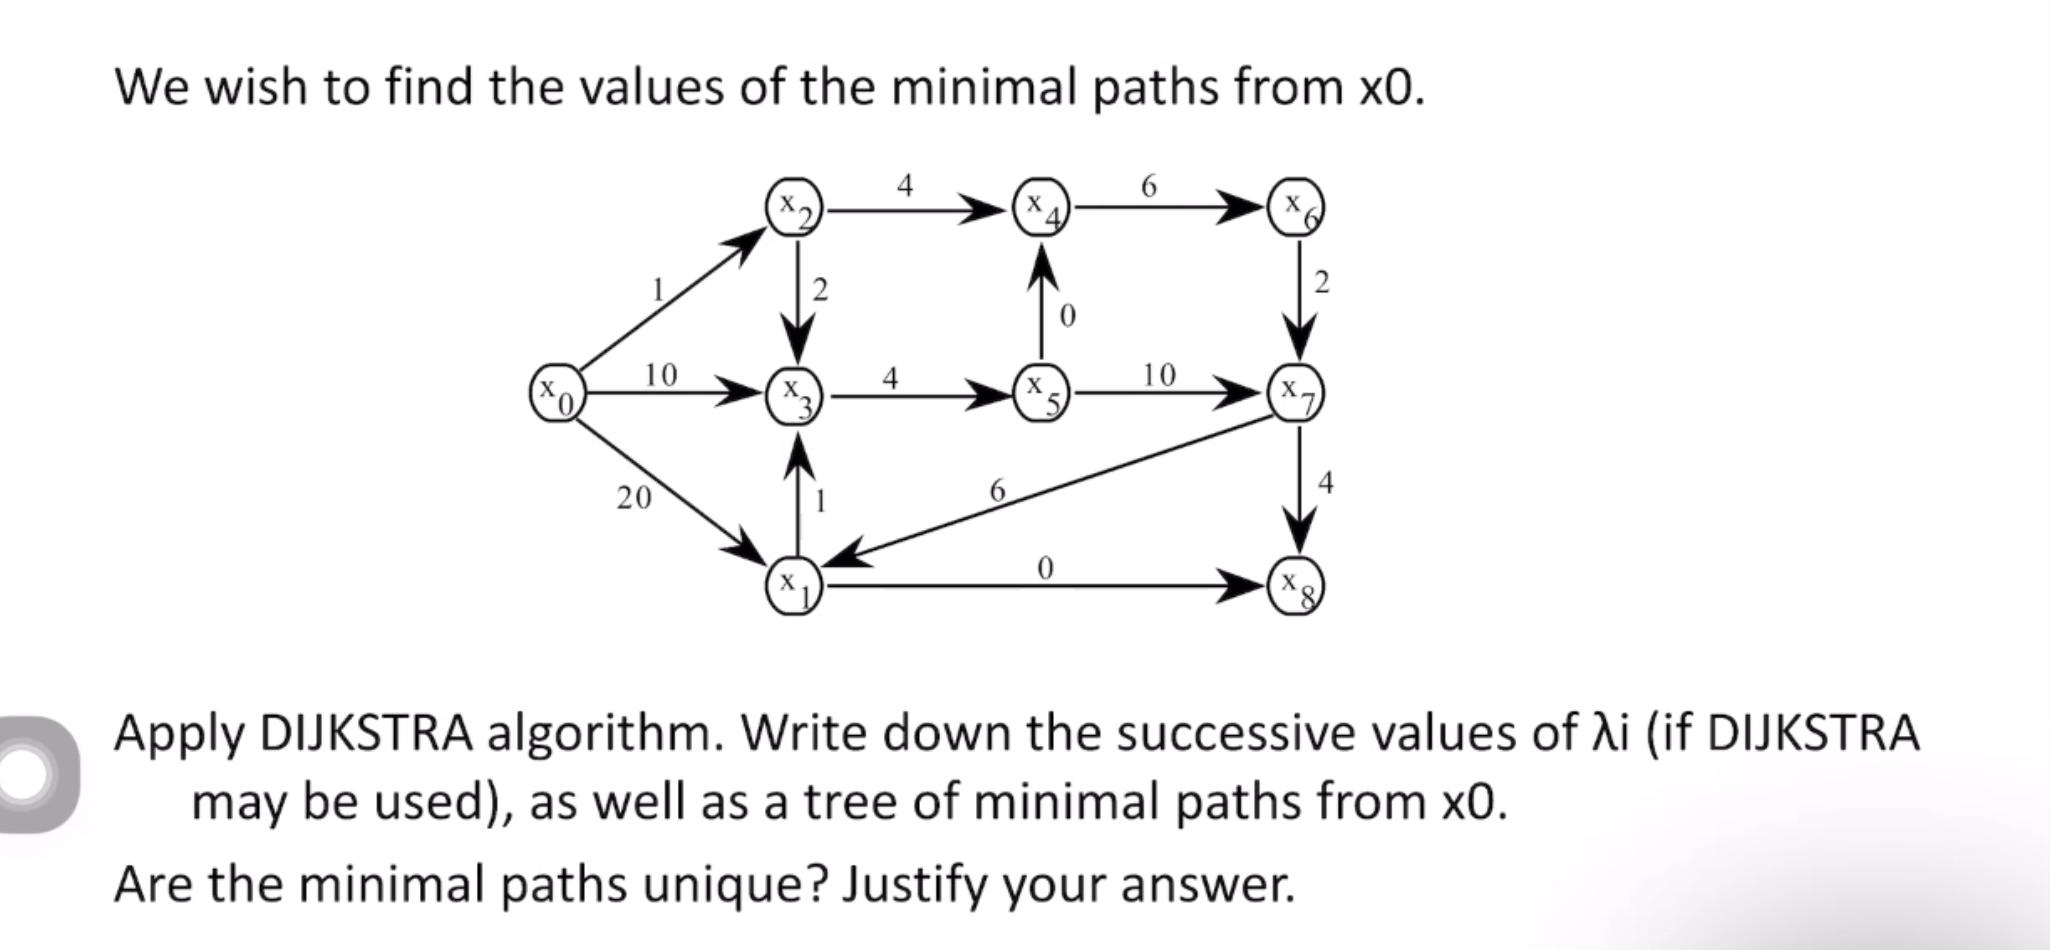
\includegraphics[width=1\textwidth]{../../images/djikstra_exercise.png}}
  \caption{}
  \label{fig:djikstra_exercise}
\end{figure}

\begin{table}[htbp]
    \centering
    \begin{tabular}{c|ccccccccc}
        Step & $x_0$ & $x_1$ & $x_2$ & $x_3$ & $x_4$ & $x_5$ & $x_6$ & $x_7$ & $x_8$\\
        \hline
        0 (start) & 0 & $\infty$ & $\infty$ & $\infty$ & $\infty$ & $\infty$ & $\infty$ & $\infty$ & $\infty$\\
        1 ($x_0$) & 0 & 20 & 1 & 10 & $\infty$ & $\infty$ & $\infty$ & $\infty$ & $\infty$\\
        2 ($x_2$) & 0 & 20 & 1 & 3 & 5 & $\infty$ & $\infty$ & $\infty$ & $\infty$\\
        3 ($x_3$) & 0 & 20 & 1 & 3 & 5 & 7 & $\infty$ & $\infty$ & $\infty$\\
        4 ($x_4$) & 0 & 20 & 1 & 3 & 5 & 7 & 11 & $\infty$ & $\infty$\\
        5 ($x_5$) & 0 & 20 & 1 & 3 & 5 & 7 & 11 & 17 & $\infty$\\
        6 ($x_6$) & 0 & 20 & 1 & 3 & 5 & 7 & 11 & 13 & $\infty$\\
        7 ($x_7$) & 0 & 19 & 1 & 3 & 5 & 7 & 11 & 13 & 17\\
        8 ($x_8$) & 0 & 19 & 1 & 3 & 5 & 7 & 11 & 13 & 17\\
        9 ($x_1$) & 0 & 19 & 1 & 3 & 5 & 7 & 11 & 13 & 17\\  
    \end{tabular}
    \caption{Dijkstra's Algorithm}
    \label{tab:dijkstra}
\end{table}

\section{Tuesday May 5th}
\subsection{Maximum Flow}
\subsubsection{Exercise 1.1}
Let $N$ be the maximum number of cars per hour which can circulate this network.

\textbf{Calculate N:} the number of maximum number of cars per hour is 41.

\section{Wednesday May 6th}
\subsection{Linear Programming}
\subsubsection{Production Example}

\begin{align}
  \text{maximize} & \quad \textbf{f}^\top \textbf{x} \\
  \text{subject to} & \quad \textbf{A} \textbf{x} \preceq \textbf{b} \\
  & \quad \textbf{x} \succeq \textbf{0}
\end{align}

\begin{align}
  \text{maximize} & \quad f \\
  \text{subject to} & \quad f = \sum_{j\in U^{+}(S)} x_{sj} - \sum_{j\in U^{-}(S)} x_{js}\\
  & \quad 
\end{align}

\section{Friday May 8th}
\subsection{Linear Programming}
\subsubsection{Exercise 7}
A computer manufacturer must plan production over $n$ months
\begin{itemize}
    \item $d_i$ = demand in month $i$
    \item $r$ = regular-time capacity per month
    \item 
\end{itemize}

\section{Studying for Final Exam}
\subsection{2025 Exam Working}
\subsubsection{Exercise 1}

\subsubsection{Exercise 2}

\subsubsection{Exercise 3}
A farmer has a limited arable land area available and wishes to organize the production of two crops (e.g., tomatoes and peppers) in order to maximize his profit. Each crop requires a certain number of working hours and a certain amount of water, both available in limited quantities for the season. Furthermore, quotas may limit the area planted with one of the crops to respond to market conditions.
The data is as follows:
 
He has a total of 20 hectares of land, 180 working hours, and 32 cubic meters of water.
1 hectare of tomatoes requires 5 working hours, 4 cubic meters of water, and yields a profit of 4 monetary units.
1 hectare of peppers requires 8 working hours, 2 cubic meters of water, and yields a profit of 6 monetary units.
To stabilize the market, he cannot plant more than 6 hectares of tomatoes.

Provide the linear programming formulation for the above problem. Propose the decision variables, the objective function, and the constraints.

\textbf{Solution: }
For this problem, the quantity we seek to maximize is $p$, the total profit of the problem.
This profit comes from the sales of tomatoes and peppers, of which the unit profit is provided for each.
We define decision variables $x_1, x_2$ as the number of tomato and pepper hectares produced respectively.
We seek to maximize the following:
\begin{equation}
    p = 4 x_1 + 6 x_2
\end{equation}
There are also a few constraints associated with land, labor, water, non-negativity, and an additional tomato constraint.
We get the following LP:

\begin{align}
  \text{maximize} & \quad 4x_1 + 6x_2 \\
  \text{subject to} & \quad x_1 + x_2 \leq 20 \\
  & \quad 5 x_1 + 8 x_2 \leq 180 \\
  & \quad 4 x_1 + 2 x_2 \leq 32 \\
  & \quad x_1 \leq 6 \\
  & \quad x_1, x_2 \geq 0
\end{align}


\end{document}
